\subsection{Lasso regression}

Our last selection method is the lasso regression. In \Fig~\ref{fig:LassoCoefVsLambda} is shown the coefficients' behavior as $\lambda$ increases. 

\begin{figure}[H]
	\centering
	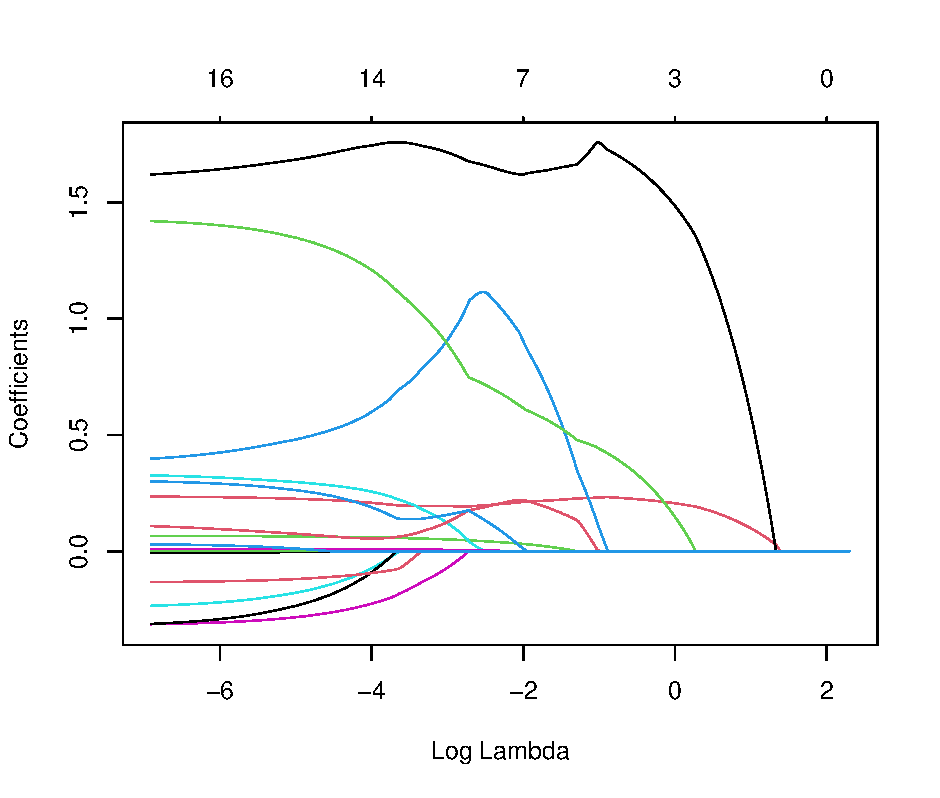
\includegraphics[width=0.4\linewidth]{ImageFiles/Regression/Lasso/LassoCoefVsLambda}
	\caption{Lasso regression coefficients as function of $\lambda$.}
	\label{fig:LassoCoefVsLambda}
\end{figure}

The same procedure followed for the ridge is applied again. In \Fig~\ref{fig:LassoCvPlot} it is possible the trend of the cross validated MSE when $\lambda$ increases. The optimal value was found to be $\lambda_{opt} = 0$, that means no penalization. The result is coherent with what obtained from Ridge Regression.

\begin{figure}[H]
	\centering
	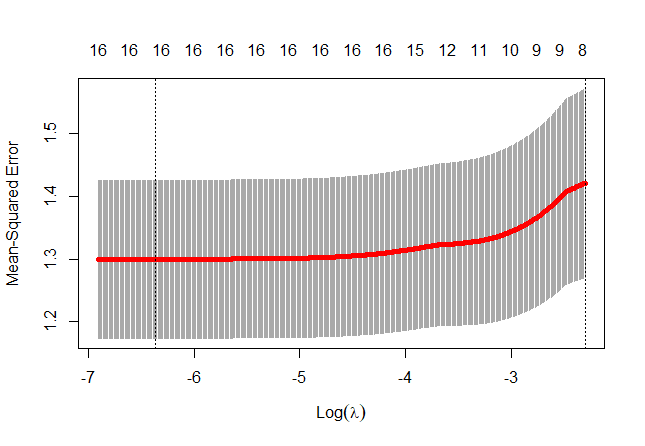
\includegraphics[width=0.5\linewidth]{ImageFiles/Regression/Lasso/LassoCvPlot}
	\caption{Lasso cross validated MSE as function of $\lambda$.}
	\label{fig:LassoCvPlot}
\end{figure}

From our analysis, it appears that penalization is not helpful in improving the model's performance for our specific use case.